% **************************************************
% Document Class Definition
% **************************************************
\documentclass[%
    paper=A4,               % paper size --> A4 is default in Germany
    ngerman,
    parskip=half,           % spacing value / method for paragraphs
    11pt,                   % font size
    headings=normal,        % size of headings
    bibliography=totoc,     % include bib in toc
    listof=totoc,           % include listof entries in toc
    chapterprefix=false,    % do not display a prefix for chapters
    appendixprefix=false,   % but display a prefix for appendix chapter
    draft=false,            % value for draft version
]{scrartcl}%

% !TeX root = handout.tex


% **************************************************
% Files' Character Encoding
% **************************************************
\PassOptionsToPackage{utf8}{inputenc}
\usepackage[T2A,T1]{fontenc}
\usepackage{inputenc}
\usepackage{booktabs}
\usepackage{minted}
\usepackage{makecell}
\usepackage{multirow}
\usepackage{todonotes}
\usepackage{caption}
\usepackage{subcaption}
\usepackage{placeins}
\usepackage{afterpage}
\usepackage{pdflscape}
\usepackage{amssymb}
\usepackage{pifont}
\usepackage{xcolor}
\usepackage{pgfplots}
\usepackage{pgfplotstable}
\usepackage{tikz}
\usepackage{enumitem}
\usepackage{footnote}
\makesavenoteenv{tabular}
\makesavenoteenv{table}
\setlist[itemize]{noitemsep, topsep=0pt}
\setlist[description]{noitemsep, topsep=0pt}
\setlist[enumerate]{noitemsep, topsep=0pt}
\usepackage{epstopdf}
\usepackage{ifthen}
\epstopdfsetup{update} % only regenerate pdf files when eps file is newer


\usepgfplotslibrary{colorbrewer}



% % show extra short titlepage
% \newif\ifShowExtraTitlePage
% \ShowExtraTitlePagetrue % enable extra titlepage
% %\ShowExtraTitlePagefalse % disable extra titlepage

% % show version on extra short titlepage
% \newif\ifShowVersionOnExtraTitlePage
% %\ShowVersionOnExtraTitlePagetrue % enable version on extra titlepage
% \ShowVersionOnExtraTitlePagefalse % disable version on extra titlepage

% % show Sperrvermerk -- ONLY required when cooperating with a company
% \newif\ifShowSperrvermerk
% \ShowSperrvermerktrue % enable 
%\ShowSperrvermerkfalse % disable

% **************************************************
% Information and Commands for Reuse
% **************************************************


\definecolor{gray}{HTML}{B8B8B8}
\definecolor{TEAL}{HTML}{298C8C}
\definecolor{MAGENTA}{HTML}{800074}
\definecolor{bblue}{HTML}{4F81BD}
\definecolor{rred}{HTML}{C0504D}
\definecolor{ggreen}{HTML}{9BBB59}
\definecolor{ppurple}{HTML}{9F4C7C}
\definecolor{oorange}{HTML}{9F7F4C}

\definecolor{indoEuropean}{HTML}{8D9BB3}
\definecolor{sinoTibetan}{HTML}{B38D8D}
\definecolor{afroAsiatic}{HTML}{8DB392}
\definecolor{turkic}{HTML}{CAD1DC}
\definecolor{dravidian}{HTML}{DCCACA}
\definecolor{japonic}{HTML}{CADCCD}

\newcommand{\mystar}{\ensuremath{\star}}
\newcommand{\thesisTitle}{Die Zukunft des Datenmanagements? Data Spaces am Beispiel von Solid} 
\newcommand{\thesisName}{Nico Schramm}
\newcommand{\thesisSubject}{Handout}
\newcommand{\thesisDate}{2025-05-25}
\newcommand{\thesisVersion}{Draft (0.1.0)}
\newcommand{\gtriuparrowred}{\textcolor{red}{$\blacktriangle$}}
\newcommand{\gtridownarrowred}{\textcolor{red}{$\blacktriangledown$}}
\newcommand{\thesisFirstReviewer}{Prof. Dr. rer. nat. Andreas Both}
\newcommand{\thesisFirstReviewerUniversity}{\protect{HTWK Leipzig}}
\newcommand{\thesisFirstReviewerDepartment}{Fakultät Informatik und Medien}
\newcommand{\numOfThesisPapers}{9\xspace} %%% DELETE
\newcommand{\numOfAThesisPapers}{2\xspace}  %%% DELETE
\newcommand{\thesisSecondReviewer}{... ...}
\newcommand{\thesisSecondReviewerUniversity}{\protect{Leipzig University of Applied Sciences}}
\newcommand{\thesisSecondReviewerDepartment}{Faculty of Computer Science and Media}
\newcommand{\thesisThirdReviewer}{... ...}
\newcommand{\thesisThirdReviewerUniversity}{\protect{... ...}}
\newcommand{\thesisThirdReviewerDepartment}{... ...}

\newcommand{\thesisFirstSupervisor}{Prof. Dr. rer. nat. Andreas Both}
\newcommand{\thesisSecondSupervisor}{... ...}

\newcommand{\thesisUniversity}{\protect{Hochschule für Technik, Wirtschaft und Kultur Leipzig}}
\newcommand{\thesisUniversityDepartment}{Fakultät für Informatik und Medien}
\newcommand{\thesisUniversityInstitute}{...}
\newcommand{\thesisUniversityGroup}{...}
\newcommand{\thesisUniversityCity}{Leipzig}
\newcommand{\thesisUniversityStreetAddress}{...}
\newcommand{\thesisUniversityPostalCode}{...}


\newcommand{\CompanyName}{}
\newcommand\Sperrvermerk[1]{
	\ifthenelse{
		#1 < 2
	}{
            \def\istgesperrt{False}
	}{
            \def\istgesperrt{True}
            \def\sperrdauer{#1}
	}
}
\def\istgesperrt{False}
%%%%%%%%%%%%%%%%%%%%%%%%%%%%%%%%%%%%%%%%%%%%%%%%%%%%%%

\newcommand{\code}[1]{\texttt{#1}}
\newcommand{\todoinline}[1]{\todo[inline]{#1}}
\newcommand{\rarrow}{\ensuremath{\rightarrow}\xspace}
\newcommand{\blind}[1]{\texttt{\lipsum[#1]}}
\usepackage[misc,geometry]{ifsym}
\usepackage{xspace}
\usepackage{amsmath}
\newcommand{\cmark}{\ding{51}}%
\newcommand{\xmark}{\ding{55}}%
\newcommand{\ie}{i.e.,\xspace}
\newcommand{\myetal}{et al.\xspace}
\newcommand{\st}{s.t.,\xspace} %% because of soul package
\newcommand{\eg}{e.g.,\xspace}
\newcommand{\wrt}{w.r.t.\xspace}
\newcommand{\egPlain}{, e.g.\xspace}
\newcommand{\Eg}{For example,\xspace}
\newcommand{\cf}{cf.\xspace}
\newcommand{\etc}{etc.\xspace}
\newcommand{\qq}[1]{``#1''}
\newcommand{\gqq}[1]{\glqq#1\grqq}
\newcommand{\num}[1]{(#1)}
\newcommand{\QAnswer}{QAnswer\xspace}
\newcommand{\QALD}{QALD\xspace}
\newcommand{\gtriuparrow}{\textcolor{green}{$\blacktriangle$}}
\newcommand{\UTQA}{UTQA\xspace}
\newcommand{\GERBIL}{GERBIL\xspace}
\newcommand{\KGQAgent}{$\mathcal{KGQA}gent$\xspace}
\newcommand{\mKGQAgent}{mKGQAgent\xspace}
\newcommand{\SimpleAgent}{$\mathcal{SA}gent$\xspace}
\newcommand{\mSimpleAgent}{mSAgent\xspace}
\newcommand{\Tool}{\textsc{Tool}\xspace}
\newcommand{\Plan}{\textsc{Plan}\xspace}
\newcommand{\ICL}{\textsc{ICL}\xspace}
\newcommand{\Env}{\textsc{Env}\xspace}
\newcommand{\WebQuestions}{WebQuestions\xspace}
\newcommand{\SimpleQuestions}{SimpleQuestions\xspace}
\newcommand{\CogComp}{TREC\xspace}
\newcommand{\TagMe}{TAGME}
\newcommand{\DBpedia}{DBpedia\xspace}
\newcommand{\Fscore}{F1 score\xspace}
\newcommand{\Fscores}{F1 scores\xspace}
\newcommand{\AnswerValidation}{\AV}
\newcommand{\NameOfNewMetrics}{Answer Trustworthiness Score\xspace}
\newcommand{\NameOfNewMetricsAtOne}{Answer Trustworthiness Score@1\xspace}
\newcommand{\NameOfNewMetricsMath}{\ensuremath{ATS}}
\newcommand{\NameOfNewMetricsMathAtOne}{\ensuremath{ATS@1}}
\newcommand{\QVmath}{\ensuremath{\QV}}
\newcommand{\QV}{\AV}
\newcommand{\QVs}{\AVs}
\newcommand{\QueryValidator}{\QV}
\newcommand{\QueryValidators}{\QVs}
\newcommand{\EAT}{EAT\xspace}
\newcommand{\NER}{NER\xspace}
\newcommand{\NEL}{NEL\xspace}
\newcommand{\NED}{NED\xspace}
\newcommand{\RE}{RE\xspace}
\newcommand{\REL}{REL\xspace}
\newcommand{\QB}{QB\xspace}
\newcommand{\QE}{QE\xspace}
\newcommand{\LLM}{LLM\xspace}
\newcommand{\MT}{MT\xspace}
\newcommand{\LM}{LM\xspace}
\newcommand{\LMs}{LMs\xspace}
\newcommand{\LLMs}{LLMs\xspace}
\newcommand{\DNNs}{DNNs\xspace}
\newcommand{\RNN}{RNN\xspace}
\newcommand{\RNNs}{RNNs\xspace}
\newcommand{\NNs}{NNs\xspace}
\newcommand{\NN}{NN\xspace}
\newcommand{\LSTM}{LSTM\xspace}
\newcommand{\GRU}{GRU\xspace}
\newcommand{\QA}{QA\xspace}
\newcommand{\NLP}{NLP\xspace}
\newcommand{\KB}{KB\xspace}
\newcommand{\URI}{URI\xspace}
\newcommand{\RESOURCE}{RESOURCE}
\newcommand{\NUMERIC}{NUMERIC}
\newcommand{\BERT}{BERT\xspace}
\newcommand{\BOOLEAN}{BOOLEAN}
\newcommand{\AV}{QV\xspace}
\newcommand{\AVs}{QVs\xspace}
\newcommand{\MRC}{MRC\xspace}
\newcommand{\NEAMT}{NEAMT\xspace}
\newcommand{\LFQA}{Lingua Franca\xspace}
\newcommand{\DATETIME}{DATETIME}
\newcommand{\LOCATION}{LOCATION}
\newcommand{\GloVe}{GloVe\xspace}
\newcommand{\Platypus}{Platypus\xspace} 
\newcommand{\DeepPavlov}{DeepPavlov\xspace}
\newcommand{\ELMo}{ELMo\xspace}
\newcommand{\wordtovec}{word2vec\xspace}
\newcommand{\MachineTranslation}{Machine Translation\xspace}
\newcommand{\HelsinkiNLP}{OPUS MT\xspace}
\newcommand{\BLEU}{BLEU\xspace}
\newcommand{\NIST}{NIST\xspace}
\newcommand{\ODQA}{OpenQA\xspace}
\newcommand{\Precision}{Precision\xspace}
\newcommand{\Recall}{Recall\xspace}
\newcommand{\KBQA}{KBQA\xspace}
\newcommand{\IRQA}{IRQA\xspace}
\newcommand{\KGQA}{KGQA\xspace}
\newcommand{\mKGQA}{mKGQA\xspace}
\newcommand{\KG}{KG\xspace}
\newcommand{\NL}{NL\xspace}
\newcommand{\IR}{IR\xspace}
\newcommand{\KGs}{KGs\xspace}
\newcommand{\QALDplus}{QALD-9-plus\xspace}
\newcommand{\RDF}{RDF\xspace}
\newcommand{\WDaquaZero}{WDAqua-core0\xspace}
\newcommand{\WDaquaOne}{WDAqua-core1\xspace}
\newcommand{\RuBQ}{RuBQ\xspace}
\newcommand{\FakeQA}{MemQA\xspace}
\newcommand{\DistilBERT}{DistilBERT\xspace}
\newcommand{\Mistral}{Mistral-7B\xspace}
\newcommand{\MISTRAL}{\Mistral}
\newcommand{\ZEPHYR}{ZEPHYR-7B\xspace}
\newcommand{\FilteringMethod}{\ensuremath{F}}
\newcommand{\isCorrect}{\ensuremath{isCorrect}}


\newcommand{\ATS}{\NameOfNewMetrics}
\newcommand{\ModelGroupOne}{$MG_1$\xspace}
\newcommand{\ModelGroupTwo}{$MG_2$\xspace}
\newcommand{\ModelGroupThree}{$MG_3$\xspace}
\newcommand{\StageOne}{$S_1$\xspace}
\newcommand{\StageTwo}{$S_2$\xspace}
\newcommand{\real}{\textit{real}\xspace}
\newcommand{\predicted}{\textit{predicted}\xspace}
\newcommand{\afterfilter}{\textit{after filtering}\xspace}
\newcommand{\beforefilter}{\textit{before filtering}\xspace}
\newcommand{\Real}{\textit{Real}\xspace}
\newcommand{\Predicted}{\textit{Predicted}\xspace}
\newcommand{\Afterfilter}{\textit{After filtering}\xspace}
\newcommand{\Beforefilter}{\textit{Before filtering}\xspace}

\newcommand{\an}[1]{\textcolor{red}{AN: #1}}
\newcommand{\numOfInitialPapers}{1875\xspace}
\newcommand{\finalNumOfSystemPapers}{27\xspace}
\newcommand{\finalNumOfDatasetPapers}{14\xspace~}
\newcommand{\finalNumOfSurveyPapers}{7\xspace~} 
\newcommand{\finalNumOfAcceptedPapers}{48\xspace}
\newcommand{\finalNumOfUniqueSystems}{22\xspace} 
\newcommand{\shareOfIndoEuropeanLangs}{88\%\xspace} 
\newcommand{\percentageOfEnglishContentOnTheWeb}{49.2\%\xspace} 
\newcommand{\percentageOfEnglishSpeakersOnTheWeb}{25.9\%\xspace} 
\newcommand{\percentageOfEnglishContentOnTheWebDE}{49.2$\;$\%\xspace} 
\newcommand{\percentageOfEnglishSpeakersOnTheWebDE}{25.9$\;$\%\xspace}

 
% Abbrevations
\newcommand{\RTE}{RTE\xspace}
\newcommand{\SOA}{SOA\xspace}
\newcommand{\QAKIS}{QAKiS\xspace}
\newcommand{\Rho}{\mathrm{P}}
\newcommand{\SPARQL}{SPARQL\xspace}
\newcommand{\LCQuAD}{LC-QuAD\xspace}
\newcommand{\LCQuADmath}{\ensuremath{\text{LC-QuAD}}}
\newcommand{\RUBQ}{RuBQ 2.0\xspace}
\newcommand{\RUBQmath}{\ensuremath{\text{RuBQ}}}
\newcommand{\EndToEndQA}{End-to-end QA\xspace}
\newcommand{\Freebase}{Freebase\xspace}
\newcommand{\Wikidata}{Wikidata\xspace}
\newcommand{\customTabular}[1]{\begin{tabular}[c]{@{}c@{}} #1\end{tabular}}
\newcommand{\CyrillicText}[1]{{\fontencoding{T2A}\selectfont #1}}
\newcommand{\dbo}[1]{\href{http://dbpedia.org/ontology/#1}{\texttt{dbo:#1}}}
\newcommand{\dbr}[1]{\href{http://dbpedia.org/resource/#1}{\texttt{dbr:#1}}}
\newcommand{\owl}[1]{\href{https://www.w3.org/2001/sw/wiki/#1}{\texttt{owl:#1}}}
\newcommand{\RQ}[1]{$\mathcal{RQ}$\textit{\thechapter.#1}}
\newcommand{\RG}[1]{$\mathcal{RG}$\textit{#1}}
\newcommand{\contribution}[1]{(\textit{#1})}

% **************************************************
% Debug LaTeX Information
% **************************************************
%\listfiles


% **************************************************
% Load and Configure Packages
% **************************************************
%\usepackage[english]{babel} % babel system, adjust the language of the content
\usepackage[ngerman]{babel}
\PassOptionsToPackage{% setup clean thesis style
    figuresep=colon,%
    hangfigurecaption=false,%
    hangsection=true,%
    hangsubsection=true,%
    sansserif=false,%
    configurelistings=true,%
    colorize=full,%
    colortheme=bluemagenta,%
    configurebiblatex=true,%
    bibsys=bibtex,%
    bibfile=references,%
    bibstyle=numeric,%
    bibsorting=nty,%
}{cleanthesis}
\usepackage{cleanthesis}

\hypersetup{% setup the hyperref-package options
    pdftitle={\thesisTitle},    %   - title (PDF meta)
    pdfsubject={\thesisSubject},%   - subject (PDF meta)
    pdfauthor={\thesisName},    %   - author (PDF meta)
    plainpages=true,           %   -
    colorlinks=false,           %   - colorize links?
    pdfborder={0 0 0},          %   -
    breaklinks=true,            %   - allow line break inside links
    bookmarksnumbered=true,     %
    bookmarksopen=true          %
}

\usepackage[table]{xcolor}
\usepackage{algorithm}
%\usepackage{algorithmic}
\usepackage{algpseudocode}

\renewcaptionname{ngerman}{\figurename}{Abb.}
\renewcaptionname{ngerman}{\tablename}{Tab.}

\addto\extrasngerman{\renewcommand\figureautorefname{Abb.}}

\usepackage{lipsum}
\usepackage{kantlipsum}
\usepackage{blindtext}

\usepackage{enumitem}
\setlist[itemize]{leftmargin=*}


\title{Die Zukunft des Datenmanagements?\\Data Spaces am Beispiel von Solid}
\author{Nico Schramm}
\date{\today}

\begin{document}

\maketitle
\thispagestyle{headings}


% content
% !TeX root = ../handout.tex

\section{Einleitung und Motivation}

\begin{itemize}
    \item aktueller Stand
    \begin{itemize}
        \item zentralisiert
        \item Datensilos, Datenmissbrauch, veraltete Daten
    \end{itemize}
    
    \item industrieller Kontext
    \begin{itemize}
        \item Daten als strategische Ressource
        \item Supply Chain (Act) Bedenken beim Teilen von Daten
    \end{itemize}

    \item Vision
    \begin{itemize}
        \item ad"=hoc"=Zusammenschaltung von Geschäftsprozessen, Daten"= / Anwendungsintegration
        \item Aktualität und Konsistenz von Daten
        \item Kostenreduktion, Wirtschaftlichkeit
        \item Vertrauen
    \end{itemize}
\end{itemize}

\cite{sambraSolidPlatformDecentralized2016,bothSolidBasedB2BData2025,mecklerWebLinkedData2023,mollerIndustrialDataEcosystems2024}

% (kurze Zusammenfassung der Struktur der Belegarbeit)
% Diese Arbeit ist folgendermaßen strukturiert. 
% In Kapitel ... 
% ...
% ...
% Abschließend ...

% !TeX root = ../notes.tex

\section{Data Spaces und Data Ecosystems}

\begin{itemize}
    \item \hl{Herleitungsketten: welche Ziele sind von jeweiligen Punkten erfüllt, was fehlt noch, von Zielen ableiten}
    \item \hl{Vergleich Solid vs. Gaia-X}
    \begin{itemize}
        \item ad-hoc, Kosten, Automatisierung, Integration
        \item Solid: einfache Integration via wohldefinierte HTTP (Standard)
        \item Gaia-X: benötigt neuen Adapter
    \end{itemize}
\end{itemize}


\subsection{Datenaustausch für Lieferketten}

\textbf{Data Sharing}
\begin{itemize}
    \item Data Sharing seit über 40 Jahren Bestandteil der Forschung
    \begin{itemize}
        \item Data Sharing: Prozess bei dem anderen Zugriff auf Daten gegeben wird, auf welche sie sonst nicht selbst Zugriff hätten
    \end{itemize}
    \item Daten für nahezu alle Geschäftsprozesse notwendig
    \item früh: versch. Vorteile von \emph{Information Partnerships} erkannt, bspw. geteilte Kosten, Verteilung von Überkapazitäten durch gemeinsame Nutzung von Kundendaten
    % \item hohe Integrationskosten, nur für reiche Unternehmen zugänglich
    \item v.a. für Koordination von Lieferketten essentiell
    \item Entgegenwirken von Fluktuationen in der Lieferkette nur mit Datenbasis möglich~\cite{mollerIndustrialDataEcosystems2024}
\end{itemize}

\vspace{1cm}

\textbf{Lieferketten}
\begin{itemize}
    \item starke Einschränkung der geteilten Daten und Informationen
    \item sehr \emph{spezifische} Daten in \emph{bilateralen} Beziehungen
    \item Data Sharing nur für bestimmten Zweck: Eindämmung negativer Effekte in Lieferketten
    \item Angst vor Missbrauch oder Verletzung der Vertraulichkeit
    \item \emph{Information Asymmetry}
    \item keine Daten teilen $\to$ Verluste, ineffiziente Lieferketten $\to$ keine Option
    \item Data Sharing benötigt Vertrauen in Wahrheitsgehalt geteilter Daten~\cite{mollerIndustrialDataEcosystems2024}
\end{itemize}


\subsection{Industrielle Data Ecosystems}

\begin{itemize}
    \item Erscheinung digital transformierter Systeme an Unternehmen
    \item alternative Sicht zu zwischenbetrieblichem Data Sharing
    \item dynamisches Data Sharing basierend auf gemeinsamen Werten (statt nur Geschäftsprozessen)
    \item Entwicklung um einen geteilten Zweck, dynamisch
    \item Gleichgewicht zwischen erhaltenem und gegebenem Aufwand (vgl. Information Asymmetry)
    \item autonome multilaterale Akteure
    \begin{itemize}
        \item ergänzen sich gegenseitig
        \item schaffen Netzwerkeffekte
    \end{itemize}
    \item zwischenbetriebliches Data Sharing + Anlehnung an biologische Ökosysteme $\to$ \emph{Data Ecosystems}
    \begin{itemize}
        \item Akteure interagieren und kooperieren
        \item \enquote{Finden, Archivieren, Veröffentlichen, Konsumieren oder Wiederverwenden von Daten}
        \item Förderung von Innovation, Wertschöpfung und Schaffung neuer Geschäfts
        \item[$\Rightarrow$] Erstellen, Verwalten und Aufrechterhalten von Anreizen für Data Sharing
    \end{itemize}
    \item Kern: Beitrag jedes Akteurs
    \begin{itemize}
        \item Data User: Verwendung von Daten
        \item Data Provider: Bereitstellung / Senden von Daten
        \item Data Intermediary: Schnittstellen~\cite{mollerIndustrialDataEcosystems2024}
    \end{itemize}
\end{itemize}


\subsection{Data Sharing Infrastructure}

\begin{itemize}
    \item Data Sharing benötigt technische Infrastruktur
    \item Kategorien: basierend auf Data Intermediaries oder \emph{Inter-Organisational Information Systems} (IOIS)
\end{itemize}

\vspace{1cm}

\textbf{IOIS}
\begin{itemize}
    \item v.a. in Lieferketten
    \item Verbindung individueller Systeme von Betrieben (bspw. ERP) für bessere Integration und automatisiertem Data Sharing
    \item meist bilateral oder multilaterale Netzwerke basierend auf einem zentralen Akteur
    \item Skalierung sehr schwierig, bspw. bzgl. Datenschutz und Kontrolle (Datensouveränität)
\end{itemize}

\vspace{1cm}

\textbf{Data Spaces}
\begin{itemize}
    \item Vereinen von DI und IOIS (vgl. \autoref{fig:dual-nature-ds})
    \item geteilter Raum für Unternehmen zur Suche nach vertrauenswürdigen Quellen
    \item Antrieb für organisationsübergreifende Optimierung und Innovation
    \item ähnlich zu DI als Vermittler zwischen Data User und Data Provider
    \item Verwendung von \emph{Data Connectors}, ermöglichen bilaterales Data Sharing (vgl. IOIS)
    \item Connectors: technisch sichergestellte Datensouveränität
    \item dezentralisiert, keine zentrale Datenspeicherung, Data Provider
    \item Data Sharing erst nach erfolgreicher Verhandlung
    \item Generierung eines \emph{Trusted Pool}s an DE-Akteuren~\cite{mollerIndustrialDataEcosystems2024}
\end{itemize}

\begin{figure}
    \includegraphics[width=\textwidth]{../shared/assets/möller_dual_nature_ds.png}
    \caption{Duale Natur von Data Spaces als Data Intermediaries und IOIs~\cite{mollerIndustrialDataEcosystems2024}}
    \label{fig:dual-nature-ds}
\end{figure}

\begin{figure}
    \includegraphics[width=\textwidth]{../shared/assets/möller_iois_di_ds.png}
    \caption{Data Sharing mit IOIS, Data Intermediaries und Data Spaces~\cite{mollerIndustrialDataEcosystems2024}}
\end{figure}


\subsection{Data Spaces in Data Ecosystems}

\begin{itemize}
    \item Data Spaces als Motor für Data Ecosystems (s.o.)
    \item dezentralisierte Daten"=Infrastruktur
    \item entworfen für Datenaustausch über mehre Unternehmen hinweg
    \item möglich durch Mechanismen für sicheres und vertrauenswürdiges Data Sharing
    \item Garantie von Datensouveränität
    \begin{itemize}
        \item Data Provider entscheidet über Zugriffskontrolle und Verwendung von geteilten Daten
    \end{itemize}
    \item flexible Formen, erlaubt bestimmter Menge an Mitgliedern Zugriff auf sicheren, vertrauenswürdigen Raum für Data Sharing
    \item Einbettung in Data Ecosystems möglich~\cite{mollerIndustrialDataEcosystems2024}
\end{itemize}

\vspace{1cm}

\begin{itemize}
    \item \emph{Data Space Member}: Akteur, welcher direkt (technisch) am Datenaustausch über DS beteiligt ist
    \item \emph{Data Ecosystem Member}: Teil des Ökosystems, aber nicht direkt am Datenaustausch durch DS beteiligt
    \begin{itemize}
        \item Beitrag zu Daten
        \item Zugriff durch \emph{Data Space Connectors}
        \begin{itemize}
            \item Schnittstelle zwischen internen Systemen der DSM und des DS an sich
            \item Erweiterungen möglich, bspw. zur Interpretation und technischer Durchsetzung von \emph{Data Usage Policies}~\cite{mollerIndustrialDataEcosystems2024}
        \end{itemize}
    \end{itemize}
\end{itemize}

\begin{figure}
    \includegraphics[width=\textwidth]{../shared/assets/möller_data_ecosystem.png}
    \caption{Data Ecosystem am Beispiel von Catena-X und Mobility Data Space~\cite{mollerIndustrialDataEcosystems2024}}
\end{figure}

\textbf{Eigenschaften von Data Spaces}
\begin{itemize}
    \item verteilt
    \begin{itemize}
        \item DS sind verteilt by Design
        \item benötigen keine physikalische Datenintegration
        \item Daten bleiben bei Quelle, Zugang nur wenn notwendig
    \end{itemize}

    \item kein einheitliches Daten"=Schema notwendig
    \begin{itemize}
        \item Datenintegration auf semantischer Ebene
        \item bspw. durch einheitliche \emph{Vocabularies}
    \end{itemize}
    
    \item Datenredundanz
    \begin{itemize}
        \item durch verteilte Architektur
        \item Daten können an versch. Orten ko-existieren
    \end{itemize}
    
    \item verschachtelt und überlappend
    \begin{itemize}
        \item DS können verschachtelt oder überlappend sein
        \item Data Provider und Data User können Mitglieder versch. DS sein
        \item Data Sharing zwischen DS~\cite{mollerIndustrialDataEcosystems2024}
    \end{itemize}
\end{itemize}

\vspace{1cm}

\textbf{Data Ecosystems}
\begin{itemize}
    \item DE entstehen um einen oder mehrere föderierte DS
    \item repräsentieren gesamte kollaborative DS-Aktivitäten
    \item Realisierung gemeinsamer Ziele der Akteure
    \item DE können mehrere DS umfassen (techn. Integration mittels Schnittstellen)
    \item Ziel: überlappende DE mit verbundenen DS $\to$ verhindern Bildung von großen Daten"=Silos
    \item Governance"=Maßnahmen über alle Abstraktionsschichten möglich (DE, DS, Use Case)
    \begin{itemize}
        \item bspw. rechtliche Anforderungen, Regeln von DS, bilaterale Regeln
    \end{itemize}
\end{itemize}

\begin{figure}
    \includegraphics[width=\textwidth]{../shared/assets/möller_data_ecosystems.png}
    \caption{Verschiedene Szenarien für Data Ecosystems~\cite{mollerIndustrialDataEcosystems2024}}
\end{figure}

\vspace{1cm}

\hl{nehmen DS, da am meisten Kriterien erfüllt, Wie kann das funktionieren? $\to$ Umsetzung Solid}

% !TeX root = ../presentation.tex

\section{Solid}

% TODO: Dreiecksbild auf meisten Folien klein in Ecke für Ref.

\begin{frame}{Solid \footnotesize\cite{mecklerWebLinkedData2023}}
    \begin{columns}
        \begin{column}{0.6\textwidth}
            \begin{itemize}
                % mögliche Implementierung des Data Space Konzeptes basiert auf Solid
                \item Data Space Konzept basierend auf\\
                    \emph{Solid} (ehem. Social Linked Data)
                    % TODO: Herkunft von Social Linked Data
                \item<2-> Ziel: offene, dezentralisierte Netzwerke für souveränen Datenaustausch
                \item<3-> Definition von Protokollen für Verwaltung und Austausch von Daten, Zugriffskontrolle und Identitätsmanagement
            \end{itemize}
        \end{column}
        
        \begin{column}{0.4\textwidth}
            \begin{figure}
                
\includegraphics[width=0.5\textwidth]{./assets/solid_logo.pdf}
                \caption{Solid-Logo~\cite{solidcommunitygroupSolidemblemsvg2019}}
            \end{figure}
        \end{column}
    \end{columns}
\end{frame}


\begin{frame}{Solid II \footnotesize\cite{mecklerWebLinkedData2023}}
    \vspace{1em}
    \begin{figure}
        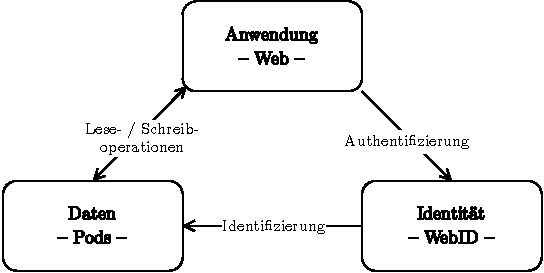
\includegraphics[height=5cm]{./assets/solid_triangle.drawio.pdf}
        \caption{Solid-Komponenten}
    \end{figure}
    % - Gliederung von Anwendungen in drei Teile
    %   - Anwendung als solches // Daten // Identität
    % - Identitätskomp.: verifiziert Identität eines Akteurs zur Auth. für Datenzugriff
    % - Daten und zugehörige Zugriffsregeln: dezentral in einen oder mehreren *Personal Online Data Stores* (Pods) gespeichert
    % - Anwendung verwendet ID, um korrekten Pod zu identifizieren und um sich für Datenzugriff zu auth.
    % - anschließend kann Anw. erforderliche Daten aus Pods lesen/schreiben
\end{frame}


\begin{frame}{Solid III \footnotesize\cite{mecklerWebLinkedData2023}}
    \begin{columns}
        \begin{column}{0.4\textwidth}
            \begin{itemize}
                \item Trennung und Standardisierung
                \item[$\Rightarrow$] Austauschbarkeit von Komponenten
                \item[$\Rightarrow$] Schritt"=für"=Schritt"=Einführung
                
                \item[$\Rightarrow$]<2-> geringe Einstiegsbarriere
                \item[$\Rightarrow$]<2-> hohe Zugänglichkeit
            \end{itemize}
        \end{column}
        
        \begin{column}{0.6\textwidth}
            \begin{figure}
                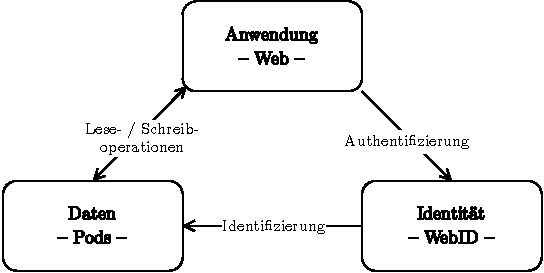
\includegraphics[width=\textwidth]{./assets/solid_triangle.drawio.pdf}
                % an Tafel malen
            \end{figure}
        \end{column}
    \end{columns}
\end{frame}


\subsection{Datenmanagement und Datenzugriff}

\begin{frame}{Datenstruktur}
    \begin{itemize}
        \item dezentrale Speicherung in \emph{Personal Online Data Stores} (Pods)~\cite{mecklerWebLinkedData2023,sambraSolidPlatformDecentralized2016}
        \item Standardisierung $\to$ Interoperabilität auf Daten"= statt Anwendungsebene
        % --> einfacher Wechsel von Anwendungen ohne aufwendige Datenmigration
        
        % \item Binärdaten\only<1|handout:0>{?} \only<2->{mit Metadaten}
        \item \only<1|handout:0>{Binärdaten?}
              \only<2>{Binärdaten mit Metadaten}
              \only<3-|handout:0>{\st{Binärdaten mit Metadaten}}
        
        \pause
        \pause
        \item lesbares Format \only<4->{$\to$ \emph{Resource Description Framework} (RDF) mit \emph{Vocabularies}~\cite{mecklerWebLinkedData2023,sambraSolidPlatformDecentralized2016}}
        % bspw. <Tim Berners-Lee> <is a> <person> (vgl. Bizer)
        % TODO: RDF-Erklärung höchstens kurz !!!
        
        \pause
        \pause
        \item Verknüpfung via \emph{Linked Data} $\to$ Struktur \& automatisierbare Semantik~\cite{bizerLinkedDataStory2009,mecklerWebLinkedData2023}

        \pause
        \item global eindeutige Identifikation via \emph{Uniform Resource Identifier} (URI)~\cite{sambraSolidPlatformDecentralized2016}
        \begin{itemize}
            \item \texttt{https://www.w3.org/People/Berners-Lee/card\#i}~\cite{bizerLinkedDataStory2009}
            % TODO: Unterschied URL / URI
        \end{itemize}
        
        \pause
        \item Zugriffskontrolle auf jeder Hierarchie-Ebene mittels \emph{Access Control List} (ACL)
        
        \pause
        \item Mapping anderer Strukturen zu RDF~\cite{mecklerWebLinkedData2023,sambraSolidPlatformDecentralized2016}
    \end{itemize}
\end{frame}


% \begin{frame}{Datenstruktur II \footnotesize\cite{mecklerWebLinkedData2023,sambraSolidPlatformDecentralized2016}}
%     \begin{columns}
%         \begin{column}{0.6\textwidth}
%             \begin{itemize}
%                 \item (nicht-) RDF"=Dateien in \emph{LDP"=Container}
%                 \item wiederum RDF"=Graph $\to$ Verschachtelung möglich
%                 \item Zugriffskontrolle auf jeder Ebene mittels \emph{Access Control List} (ACL)
%                 \begin{itemize}
%                     \item \texttt{resource.acl} oder \texttt{.acl}
%                 \end{itemize}

%                 \item<2> unterschiedliche Rechte pro Akteur / Container
%                 \item[$\Rightarrow$]<2> feingranularer Datenschutz und Zugriffskontrolle
%             \end{itemize}
%         \end{column}

%         \begin{column}{0.4\textwidth}
%             \vspace{1em}
%             \begin{figure}
%                 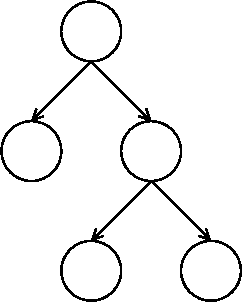
\includegraphics[height=4.5cm]{./assets/container_hierarchy.drawio.pdf}
%                 \caption{Hierarchie \cite[vgl.][]{sambraSolidPlatformDecentralized2016}}
%             \end{figure}
%         \end{column}
%     \end{columns}
% \end{frame}


\begin{frame}{Read- und Write-Protokoll \footnotesize\cite{mecklerWebLinkedData2023,sambraSolidPlatformDecentralized2016}}
    \begin{itemize}
        \item Anwendungen lesen und schreiben Daten direkt aus Pods
        \item Interoperabilität der Pods mit Anwendungen\\
            und wohldefiniertes, einfach implementierbares Protokoll
            % möglichst viel wiederverwenden, was bereits vorhanden ist
            % soll keine neue Komponenten sein --> aufbauend auf RESTful
        \item[$\Rightarrow$]<2-> RESTful"=Service, welche \emph{Linked Data Platform} (LDP) erfüllen
        \begin{itemize}
            % LDP: beschreibt Datenformat
            %   Einteilung in Ressourcen und Containern, Paging
            \item<2-> \texttt{HTTP GET}, \texttt{POST}, \texttt{PATCH}, \texttt{DELETE} etc.~\cite{sambraSolidPlatformDecentralized2016}
        \end{itemize}

        \item<3-> komplizierte Datenabfragen mittels SPARQL (optional)
    \end{itemize}
\end{frame}

% Fazit
% Datenmanagement betrachtet
% dezentrale Speicherung, Interoperabilität auf Daten- statt Anw.-Ebene
% Wie identifizieren wir Datenspeicher und Akteure für Datenzugriff? 

% \begin{frame}{Datenabfragen \footnotesize\cite{sambraSolidPlatformDecentralized2016}}
%     \begin{itemize}
%         \item nur einfache Abfragen mittels LDP"=Methoden möglich
%         \item komplizierte Datenabfragen mittels SPARQL (optional)
%         \item Delegation an Server $\Rightarrow$ Entwicklungsaufwand $\downarrow$

%         \pause
%         \item \emph{Local Queries}: innerhalb \emph{eines} Pods
%         \item \emph{Link Following Queries}: über mehrere Pods hinweg
%         \begin{itemize}
%             \item via Link"=Following
%             \item tatsächliche Verteilung muss nicht bekannt sein
%         \end{itemize}
%     \end{itemize}
% \end{frame}


\subsection{Identität und Authentifizierung}

\begin{frame}{Authentifizierung \footnotesize\cite{sambraSolidPlatformDecentralized2016}}
    \begin{itemize}
        \item Vertrauen, Datensouveränität und Datenschutz $\to$ Authentifizierung
        \item Dezentralisierung benötigt globalen \emph{Identity Space}
        
        \item<2-> passend zu RDF"=basierten Daten
        \item<2-> Ermittlung der Identität und Profildaten
        \item<2-> Ermittlung relevanter Links zum Pod und zu Anwendungsdaten
        
        \item[$\Rightarrow$]<3-> aktuell: \emph{WebID} (austauschbar)
        \item[$\Rightarrow$]<3-> globales Identitätsmanagement basierend auf System dezentralisierter \emph{Identity Provider}
    \end{itemize}
\end{frame}


\begin{frame}{Identität}
    \begin{columns}
        \begin{column}{0.55\textwidth}
            \begin{itemize}
                \item Akteure besitzen WebID"=URI~\cite{sambraSolidPlatformDecentralized2016}
                
                \item Referenz auf \emph{WebID Profile Document}~\cite{sambraSolidPlatformDecentralized2016,solidcommunitygroupSolidemblemsvg2019}
                
                \begin{itemize}
                    \item<2-> Referenz auf Pod und Anwendungsdaten~\cite{solidcommunitygroupSolidWebIDProfile2024}
                    \item<2-> Referenz auf weitere Profildaten~\cite{solidcommunitygroupSolidWebIDProfile2024}
                    % Webseite im RDF"=Format, global eindeutige URI~\cite{sambraSolidPlatformDecentralized2016}
                \end{itemize}
                
                \item<3-> Speicherung bei Identity Provider\\
                    (meist Pod Provider)~\cite{sambraSolidPlatformDecentralized2016}
                \item[$\Rightarrow$]<3-> Kontrolle über eigene Identität bei Nutzenden~\cite{sambraSolidPlatformDecentralized2016}
            \end{itemize}
        \end{column}

        \begin{column}{0.45\textwidth}
            \only<2->{
                \begin{figure}
                    \centering
                    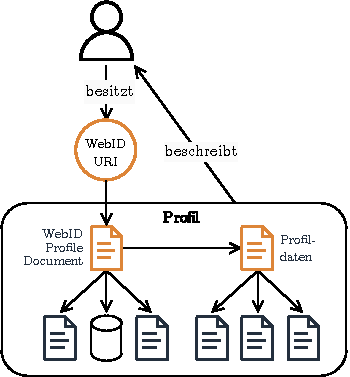
\includegraphics[height=5.5cm]{./assets/profile.drawio.pdf}
                    \caption{Solid Profil~\cite[vgl.][]{sambraSolidPlatformDecentralized2016,solidcommunitygroupSolidWebIDProfile2024}}
                \end{figure}
            }
        \end{column}
    \end{columns}
\end{frame}


\begin{frame}{Web of Trust \footnotesize\cite{sambraSolidPlatformDecentralized2016}}
    \begin{columns}
        \begin{column}{0.6\textwidth}
            \begin{itemize}
                \item Verknüpfung von Identitäten über mehrere Seiten\\
                $\Rightarrow$ \emph{Web of Trust}
                % hilfreich, da man nicht alle Akteure in einem DS / DE kennen kann
                
                \item[$\Rightarrow$]<2-> ad-hoc Auth.-Entscheidungen basierend auf Profileigenschaften
                % bspw. Beziehungen zu anderen Akteuren, Arbeitsstelle, Teil einer Gruppe etc. etc.
                % transitives Vertrauen
                
                \item[$\Rightarrow$]<3-> Wem kann ich vertrauen?\\ Kann ich den geteilten Daten vertrauen?
                
                \item[$\Rightarrow$]<4-> Adressierung eines Kern"=Hindernisses
            \end{itemize}
            % aber wenn ein Akteur kompromittiert, dann SCHLECHT
        \end{column}
        
        \begin{column}{0.4\textwidth}
            \vspace{1em}
            \begin{figure}
                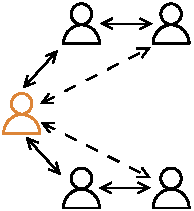
\includegraphics[height=4cm]{./assets/web_of_trust.drawio.pdf}
                \caption{Web of Trust}
            \end{figure}
        \end{column}
    \end{columns}
\end{frame}


\subsection{Erweiterung: Wertschöpfungsketten}

\begin{frame}{Erweiterung: Wertschöpfungsketten \footnotesize\cite{bothSolidBasedB2BData2025}}
    \begin{itemize}
        \item automatisierte Datenübertragung essenziell für Partner:in in Wertschöpfungsketten
        \item weitere Anforderungen
        \begin{itemize}
            \item garantierte, nachvollziehbare Einhaltung rechtlicher Rahmenbedingungen
            \item Constraints für Data Sharing
        \end{itemize}
    \end{itemize}

    \begin{figure}
        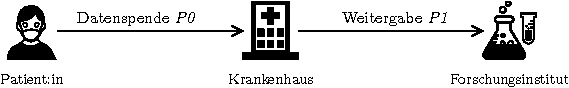
\includegraphics[width=\textwidth]{./assets/example_horizontal.drawio.pdf}
        \caption{Beispiel: Datenspende}
    \end{figure}
\end{frame}


\begin{frame}{Erweiterung: Wertschöpfungsketten II \footnotesize\cite{bothSolidBasedB2BData2025}}
    \addtocounter{figure}{-1}
    \begin{figure}
        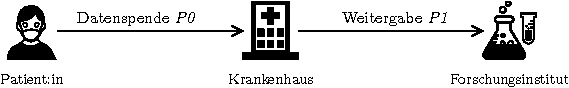
\includegraphics[width=\textwidth]{./assets/example_horizontal.drawio.pdf}
        \caption{Beispiel: Datenspende}
    \end{figure}
    
    \vspace{-1em}

    \begin{itemize}
        \item Einführung zusätzlicher Metadaten
        \begin{itemize}
            \item \emph{Data Processing Purpose} $P$ % Weitergabe muss sich trotzdem an ursprüngl. Zweck halte
            \item Verstecken der Datenquelle, Angabe über Weitergabe
        \end{itemize}

        \item<2-> weitere Validierung notwendig
        % weiterer Schritt in Richtung E2E-B2B-Wertschöpfungsketten
        % Möglichkeit und Notwendigkeit zur Erweiterung von Solid
    \end{itemize}

    % TODO: Stichpunkte zum Erzählen
\end{frame}

% !TeX root = ../handout.tex

\section{Einschätzung und Zukunft}

Die Verwendung von Solid vereint viele Ziele, um die einleitend genannte Vision näher in die Realität zu bringen.
So existiert ein Ansatz zur Gewährleistung von Datensouveränität und Datenschutz, auch wenn noch Konzepte notwendig sind, welche die Zwischenspeicherung durch Data User und somit die Bildung großer Datensilos verhindert.
Mittels Web of Trust können Authentifizierungsentscheidungen schnell und effizient getroffen werden, wodurch vertrauenswürdig Daten geteilt werden können.
Jedoch sind Ansätze gegen Kompromittierung notwendig.

Durch Standardisierung, Interoperabilität und Wiederverwendbarkeit werden Anwendungen und Daten entkoppelt, wodurch ein Wechsel ohne aufwendige Migrationen ermöglicht wird.
Gekoppelt mit der Auslagerung von Standardfunktionalitäten können Entwicklungskosten und somit Einstiegsbarrieren für neue Unternehmen gesenkt werden.
Dadurch ist mehr Wettbewerb und Innovation möglich.

Insgesamt ist das Ziel, ad-hoc Daten"= und Anwendungsintegrationen zu ermöglichen, wofür statt aufwendigen ETL"=Prozessen nur ein Mapping der Datenstrukturen vorgenommen werden muss.
Daten können von Domänen abstrahiert werden, da eine dynamische Interpretation durch die Semantik aus den RDF"=Daten möglich ist, was in Richtung Metaprogrammierung führen könnte.
Allerdings müssen die Daten vorher in entsprechenden, digitalen Formaten vorliegen.

Da die Datenstrukturen nicht mehr von den Anwendungen abhängen, wird eine andere Art und Weise der Unterscheidung auf dem Markt notwendig sein, da Unternehmen ihre Kund:innen nicht mehr durch proprietäre Datenformate halten können.
Eine Nutzerzentrierung sowie der Qualitätsanspruch könnten zunehmen, da Nutzende sonst problemlos zu anderen Alternativen wechseln könnten.
Durch eine niedrigere Einstiegshürde in den Markt würde dies begünstigt werden.

% !TeX root = ../presentation.tex

\section{Einschätzung und Zukunft}

\begin{frame}{Einschätzung}
    \begin{itemize}
        \item Zusammenführung vieler Ziele, um Vision näher an Realität zu bringen
        
        \pause
        \item Vertrauen?
        \pause
        \begin{itemize}
            \item Ansatz für Datensouveränität, Datensilos? gesetzliche Vorgaben?
        \end{itemize}
        % Ansatz zur Gewährleistung von Datensouveränität
        % unterschiedliche Datenspeicher je nach Kontext, Web of Trust
        % größerer Anreiz für Speicherung von Daten (<-- mehr Vertrauen und Kontrolle)
        % Web of Trust: ein kompromittierter Akteur reicht, um Schaden anzurichten
        % Startpunkt, aber wie verhindern, dass Data User die Daten zwischenspeichern?
        % Einhaltung gesetzlicher Vorgaben? --> o.g. Ansatz (Metadaten) benötigt weitere Forschung

        \pause
        \item Aktualität und Konsistenz von Daten?
        \pause
        \begin{itemize}
            \item Dezentralisierung und Datensouveränität, Anreiz $\uparrow$, Standardisierung
        \end{itemize}
        % mehr Vertrauen + Dezentralisierung + Datensouveränität 
        %     --> Daten bei Nutzenden
        %     --> größerer Anreiz zum Speichern von Daten
        % können diese einfach aktuell halten
        %     im Vgl. zu zentralisierten Ansatz, wo dieselben Daten verteilt bei vielen Unternehmen liegt
        % Standardisierung --> größere Verfügbarkeit von Daten

        \pause
        \item Effizienz und Geschwindigkeit?
        \pause
        \begin{itemize}
            \item Interoperabilität, automatisierbare Semantik, ggf. Mapping
        \end{itemize}
        % standardisierte Speicherung von Daten
        % Interoperabilität auf Daten- statt Anwendungsebene
        % automatisierbare Semantik durch RDF + Vocabularies
        % dadurch schnellere Datenintegration möglich, ggf. Mapping notwendig (teil- / automatisiert)

        \pause
        \item Zugänglichkeit unabhängig von Größe, Branche etc.?
        \pause
        \begin{itemize}
            \item Interoperabilität, Aufwand $\downarrow$, niedrigere Einstiegsbarriere

            \pause
            \item[$\Rightarrow$] Förderung von Kooperation und Innovation
        \end{itemize}
        % Interoperabilität auf Daten- statt Anw.-Ebene
        %     --> keine eigenen Daten mehr notwendig
        %     --> Zugänglichkeit von Daten
        % verminderter Aufwand durch Auslagerung von Std.-Fkt. + Wiederverwendbarkeit
        % niedrigere Einstiegsbarriere
        % Zugänglichkeit des Marktes
    \end{itemize}
\end{frame}


\begin{frame}{Zukunft}
    % TODO: Beispiel durchziehen
    % stellen uns vor: cooles neues Projekt
    % gehe zu neuen potenziellen Gesch.-Partnern und bringe meine Akten-Tasche voller Daten mit
    % ich kann alle meine Daten immer mit mir führen

    % dafür müssen sie digital sein

    \begin{itemize}
        \item Digitalisierung zum Profitieren von Vorteilen
        % digitales Bild nicht ausreichend, brauchen Daten mit automatisierbarer Semantik

        % interoperabel zur einfachen Zusammenführung
        \pause
        \item Dezentralisierung und Interoperabilität
        \begin{itemize}
            \item[$\to$] Fokus auf dezentrale Architekturen
        \end{itemize}

        % damit ermögliche ich ...
        \pause
        \item Ermöglichung von ad"=hoc Daten- und Anwendungsintegrationen
        \begin{itemize}
            \item[$\to$] Mapping statt aufwendige ETL"=Prozesse
                % Wiederverwendung, Schnittstellen
            
            % dyn. Interpr. durch Semantik aus RDF-Daten -->
            \item[$\to$] Abstraktion von Domänen-Daten, Metaprogrammierung
            % Branchen-agnostische Daten
            % Zukunft: Agenten interpretieren Daten nach meinen Kriterien, unabh. ob es User, Patient oder Benutzer heißt
        \end{itemize}

        % wird begünstigt durch
        \pause
        \item Datenstrukturen unabhängig von Anwendungen, Verfügbarkeit von Daten
        \begin{itemize}
            % aktuell: Wenn ich das mache, gehen Kunden weg?
            %          Einsperren von Kunden durch proprietäre Datenformate
            \item[$\to$] neue Art und Weise der Unterscheidung auf Markt
            \item[$\to$] Nutzerzentrierung, steigender Qualitätsanspruch
            % gutes Produkt zieht Kund. an, schlechtes stößt ab
            % begünstigt durch niedrigere Einstiegshürden in Markt
            % TODO: Blocker: Big Player werden dagegen wirken
        \end{itemize}

        \pause
        \item[$\Rightarrow$] Daten-orientiertes Vorgehen statt Prozess-Orientierung
        % Daten als Antreiber statt Prozesse
    \end{itemize}
\end{frame}

% !TeX root = ../handout.tex

\section{Fazit}

In diesem Handout wurden Data Spaces vorgestellt, welche dezentrale, multilaterale Informationssysteme anstreben, um ein vertrauenswürdiges Data Sharing unter Garantie von Datensouveränität zu ermöglichen.
Eine mögliche Umsetzung basiert auf dem offenen Standard Solid, welcher die Verwaltung und den Austausch von Daten und Identitäten definiert.
Daten werden dezentral in Pods gespeichert, wobei die volle Kontrolle über den Zugang bei Nutzenden liegt.
Durch Standardisierung und Interoperabilität können Datenspeicher unabhängig von Anwendungen gewechselt werden.
Authentifizierungsentscheidungen können ad-hoc über ein Web of Trust getroffen werden.
Somit soll ein vertrauenswürdiges Teilen von aktuellen und konsistenten Daten als Basis für effiziente Integrationen ermöglicht werden.
Zukünftig könnte dies in Richtung vollständige Digitalisierung, Metaprogrammierung mit agnostischen Daten sowie Nutzerzentrierung von Anwendungen führen.



{%
    \setstretch{1.1}
    \renewcommand{\bibfont}{\normalfont\small}
    \setlength{\biblabelsep}{0.25em}
    \setlength{\bibitemsep}{0.5\baselineskip plus 0.5\baselineskip}
    % print all references that are not ot type online
    \printbibliography[nottype=online]
    \newrefcontext[labelprefix={@}]
    % web pages are typically non-scientific resources, so we separate them from the scientific ones
    % typically 
    \printbibliography[heading=subbibliography,title={Webpages},type=online]
}

\listoffigures
\thispagestyle{headings}

\listoftables
\thispagestyle{headings}

%\lstlistoflistings

\end{document}
